% =====================================================================================
% Appendix to Sec. 6 (C3).  Owner: parth.  FALLBACK skeleton by ojas (branch ojas/paper-c3).
% Same macro file and helpers as 06_c3.tex (\Cres, \CresCI, \CthreePending, \Cfit).
% Labels defined: sec:c3-app, fig:c3-speed.
% The T12 sanity/cost table and the speed-1/3 rows are NOT in the paper: they go to the code
% archive's results README (parth).  NO RESULTS EXIST YET.
% Sanity design: prereg/t12_sanity.json (PR #7): Fast-dLLM's LLaDA-8B-Instruct GSM8K settings,
% lm-eval 5-shot, 200 fit-half problems, top-k k=1 (published 79.3) and threshold 0.9
% (published 79.2; Fast-dLLM Table 1, "+Parallel").  The published numbers are design constants
% here, from that file, written as fractions (0.793, 0.792) like every other number; the
% plan's bar is 0.01--0.02.  Sanity intervals are 95% Wilson.
% =====================================================================================

\subsection{C3: sanity check and speed curves (T12, exploratory)}
\label{sec:c3-app}

Before the comparison, the harness decodes \Cres{CThreeTTwelveSanityN} fit-half GSM8K
problems at Fast-dLLM's settings (5-shot, 256 tokens, blocks of 32; fp16 on an RTX 2080 Ti).
Top-$k$ at $k=1$ scores \CresCI{CThreeTTwelveSanityTopKAcc} against a published 0.793, and the
threshold rule at $\tau=0.9$ \CresCI{CThreeTTwelveSanityThresholdAcc} against 0.792
\citep{wu2025fastdllm}; intervals are 95\% Wilson.
Figure~\ref{fig:c3-speed} plots accuracy against tokens per step at all three speeds; the cost
per decoder and the speed-1 and speed-3 rows are in the code archive.
% Fast-dLLM's numbers are on the full test set, ours on 200 fit-half problems, so compare the
% interval, not the point.
% TODO(results): if both published values lie inside our Wilson intervals: "Both published
%   values lie inside our intervals, so the harness reproduces the two decoders it can be
%   checked on" (add "although our points are above them" if so).  Else: "<Decoder> scores
%   above/below the published value, which lies outside our interval: <likely cause, e.g.
%   prompt or stop-string difference, to be checked>; Sec. 6 is read with that in mind."
%   Replace the last clause of the paragraph with this sentence if space allows.

\begin{figure}[t]
  \centering
  \IfFileExists{../artifacts/t12/figures/t12_matched_speed.pdf}%
    {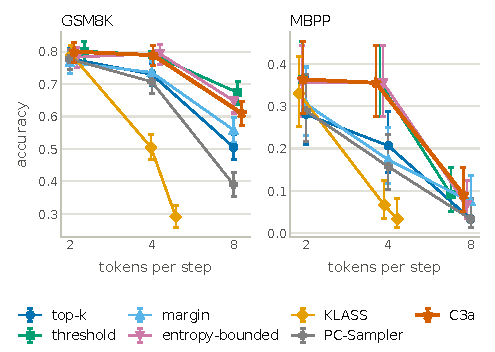
\includegraphics[width=\columnwidth]{../artifacts/t12/figures/t12_matched_speed}}%
    {\CthreePending{Figure accuracy against tokens per step}}
  \caption{Accuracy against aggregate tokens per step, one panel per task (left GSM8K, right
    MBPP), one curve per decoder at its three speeds, with 95\% Wilson intervals. Up and to the
    right is better.}
  \label{fig:c3-speed}
\end{figure}
